\documentclass[10pt, a4paper, landscape]{article}
\usepackage[left=1cm, right=1cm, top=2cm, bottom=2cm]{geometry}
\usepackage{longtable}
\usepackage{array}
\usepackage{xcolor}
\usepackage{colortbl}
\usepackage{fancyhdr}
\usepackage{lscape}
\usepackage{verbatim}
\usepackage{fancyvrb}
\usepackage{listings}
\usepackage[hidelinks]{hyperref}
\usepackage{tikz}
\usetikzlibrary{automata, positioning, arrows}

\title{\textbf{Evse.py Unit Test Report}}
\author{MEA OCPP Certification (Automated)}
\date{\today}

\pagestyle{fancy}
\fancyhf{}
\lhead{MEA Evse State Machine Verification}
\rhead{Page \thepage}

\begin{document}

\maketitle

\section*{State Transition Diagram}
\begin{center}
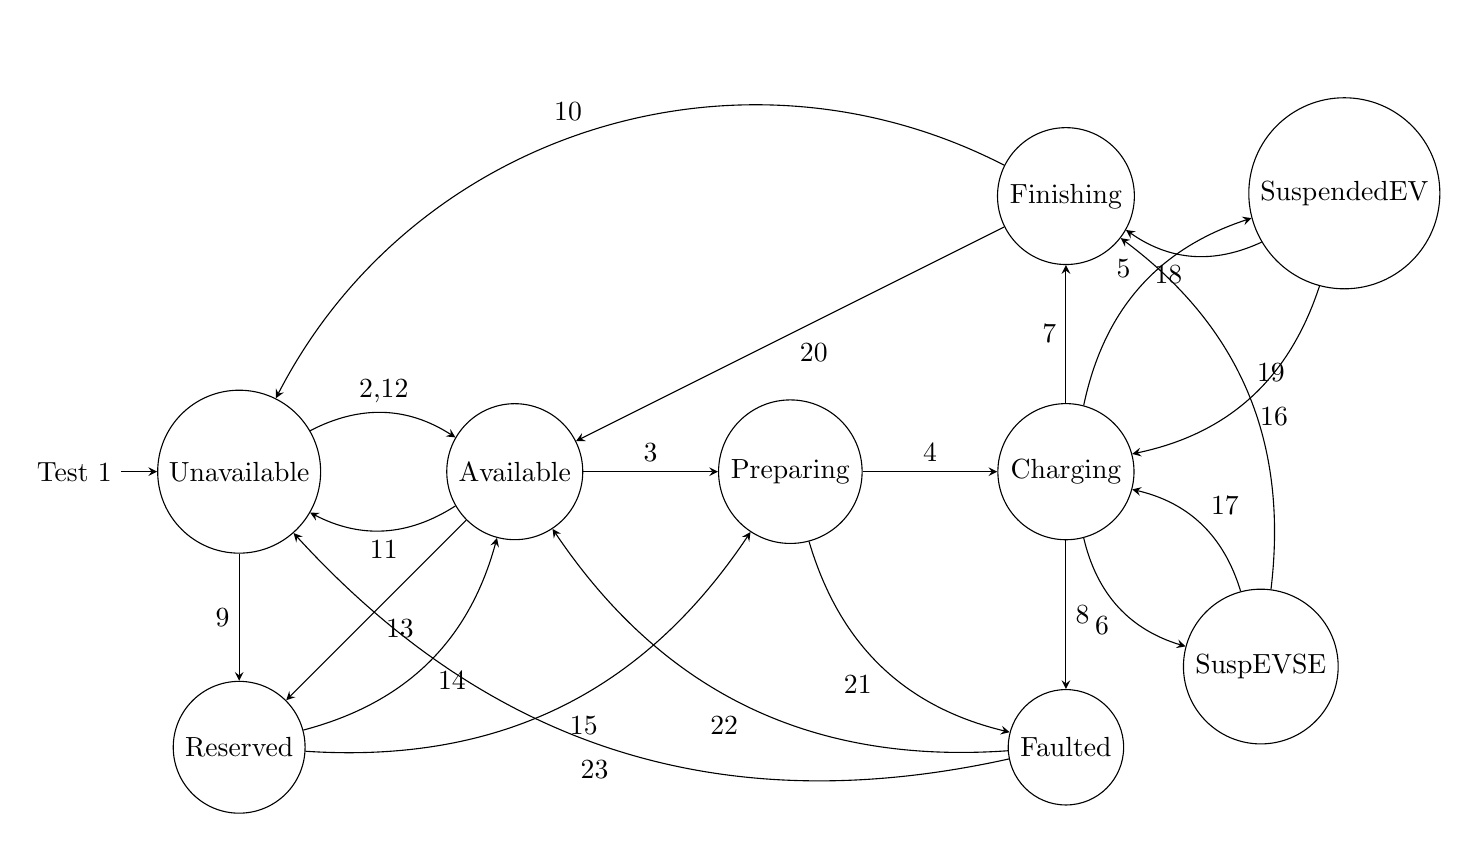
\begin{tikzpicture}[>=stealth, node distance=3.5cm, on grid, auto, initial text=Test 1]
  \node[state, initial] (unavailable) {Unavailable};
  \node[state] (available) [right=of unavailable] {Available};
  \node[state] (reserved) [below=of unavailable] {Reserved};
  \node[state] (preparing) [right=of available] {Preparing};
  \node[state] (charging) [right=of preparing] {Charging};
  \node[state] (suspendedev) [above right=5cm of charging] {SuspendedEV};
  \node[state] (suspendedevse) [below right=of charging] {SuspEVSE};
  \node[state] (faulted) [below=of charging] {Faulted};
  \node[state] (finishing) [above=of charging] {Finishing};

  \path[->]
    (unavailable) edge [bend left] node {2,12} (available)
    (available) edge [bend left] node {11} (unavailable)
    
    (unavailable) edge node [left] {9} (reserved)
    (available) edge node {13} (reserved)
    (reserved) edge [bend right] node [swap] {14} (available)
    (reserved) edge [bend right] node [swap] {15} (preparing)
    
    (available) edge node {3} (preparing)
    (preparing) edge node {4} (charging)
    (preparing) edge [bend right] node [swap] {21} (faulted)
    
    (charging) edge [bend left] node {5} (suspendedev)
    (suspendedev) edge [bend left] node {16} (charging)
    (suspendedev) edge [bend left] node {18} (finishing)
    
    (charging) edge [bend right] node [swap] {6} (suspendedevse)
    (suspendedevse) edge [bend right] node [swap] {17} (charging)
    (suspendedevse) edge [bend right] node [swap] {19} (finishing)
    
    (charging) edge node {7} (finishing)
    (charging) edge node {8} (faulted)
    
    (finishing) edge [bend right=45] node [swap] {10} (unavailable)
    (finishing) edge node {20} (available)
    
    (faulted) edge [bend left] node {22} (available)
    (faulted) edge [bend left] node {23} (unavailable);
\end{tikzpicture}
\end{center}
\vspace{1cm}

\section*{Unit Test Execution Results}

\renewcommand{\arraystretch}{1.3}
\begin{longtable}{|c|p{6cm}|p{2.5cm}|p{8cm}|c|}
\hline
\rowcolor{gray!30}
\textbf{ID} & \textbf{Test Case} & \textbf{State Check} & \textbf{Log Preview / Trace} & \textbf{Result} \\
\hline
\endfirsthead

\hline
\hline
\rowcolor{gray!30}
\textbf{ID} & \textbf{Test Case} & \textbf{State Check} & \textbf{Log Preview / Trace} & \textbf{Result} \\
\hline
\endhead

\hline
\endfoot
1 & test\_initial\_state & Logic Check & \texttt{\scriptsize WHITE-beet-EI firmware version: 1.0.0} \newline \texttt{\scriptsize RFIDSim stopped.} & \textcolor{green}{PASSED} \\
\hline
2 & test\_transition\_to\_available & Logic Check & \texttt{\scriptsize WHITE-beet-EI firmware version: 1.0.0} \newline \texttt{\scriptsize Set the CP mode to EVSE} \newline \texttt{\scriptsize Set the CP duty cycle to 100\%} \newline \texttt{\scriptsize Start the CP service} \newline \texttt{\scriptsize Start SLAC in EVSE mode} \newline \texttt{\scriptsize RFIDSim started. Call simulate\_scan(id\_tag) to trigger.} \newline \texttt{\scriptsize State transition: Unavailable -> Available} & \textcolor{green}{PASSED} \\
\hline
3 & test\_transition\_to\_preparing & Logic Check & \texttt{\scriptsize WHITE-beet-EI firmware version: 1.0.0} \newline \texttt{\scriptsize RFIDSim started. Call simulate\_scan(id\_tag) to trigger.} \newline \texttt{\scriptsize RFID Scanned: RFID\_TAG} \newline \texttt{\scriptsize EVSE Authorized by OCPP: RFID\_TAG} \newline \texttt{\scriptsize EV already connected, transitioning to Preparing for authorized tag: RFID\_TAG} \newline \texttt{\scriptsize State transition: Available -> Preparing} \newline \texttt{\scriptsize EV already connected} & \textcolor{green}{PASSED} \\
\hline
4 & test\_transition\_to\_charging & Logic Check & \texttt{\scriptsize WHITE-beet-EI firmware version: 1.0.0} \newline \texttt{\scriptsize "Energy transfer mode selected" received} \newline \texttt{\scriptsize State transition: Preparing -> Charging} \newline \texttt{\scriptsize Maximum voltage: 400} \newline \texttt{\scriptsize Maximum current: 32} \newline \texttt{\scriptsize RFIDSim stopped.} & \textcolor{green}{PASSED} \\
\hline
5 & test\_transition\_to\_suspended\_ev & Logic Check & \texttt{\scriptsize WHITE-beet-EI firmware version: 1.0.0} \newline \texttt{\scriptsize "DC Charge Parameters Changed" received} \newline \texttt{\scriptsize EV maximum current: 32A} \newline \texttt{\scriptsize EV maximum voltage: 400V} \newline \texttt{\scriptsize EV ready: True} \newline \texttt{\scriptsize Error code: 0} \newline \texttt{\scriptsize SOC: 50\%} \newline \texttt{\scriptsize EV target current: 0A} \newline \texttt{\scriptsize State transition: Charging -> SuspendedEV} \newline \texttt{\scriptsize RFIDSim stopped.} & \textcolor{green}{PASSED} \\
\hline
6 & test\_transition\_to\_suspended\_evse & Logic Check & \texttt{\scriptsize WHITE-beet-EI firmware version: 1.0.0} \newline \texttt{\scriptsize "DC Charge Parameters Changed" received} \newline \texttt{\scriptsize EV maximum current: 32A} \newline \texttt{\scriptsize EV maximum voltage: 400V} \newline \texttt{\scriptsize EV ready: True} \newline \texttt{\scriptsize Error code: 0} \newline \texttt{\scriptsize SOC: 50\%} \newline \texttt{\scriptsize EV target current: 10A} \newline \texttt{\scriptsize State transition: Charging -> SuspendedEVSE} \newline \texttt{\scriptsize RFIDSim stopped.} & \textcolor{green}{PASSED} \\
\hline
7 & test\_transition\_to\_finishing & Logic Check & \texttt{\scriptsize WHITE-beet-EI firmware version: 1.0.0} \newline \texttt{\scriptsize "Session stopped" received} \newline \texttt{\scriptsize State transition: Charging -> Finishing} \newline \texttt{\scriptsize Closure type: 0} \newline \texttt{\scriptsize RFIDSim stopped.} & \textcolor{green}{PASSED} \\
\hline
8 & test\_transition\_to\_faulted & Logic Check & \texttt{\scriptsize WHITE-beet-EI firmware version: 1.0.0} \newline \texttt{\scriptsize "Session Error" received} \newline \texttt{\scriptsize State transition: Charging -> Faulted} \newline \texttt{\scriptsize Session error: 0: Unspecified} \newline \texttt{\scriptsize RFIDSim stopped.} & \textcolor{green}{PASSED} \\
\hline
9 & test\_transition\_to\_reserved & Logic Check & \texttt{\scriptsize WHITE-beet-EI firmware version: 1.0.0} \newline \texttt{\scriptsize State transition: Unavailable -> Reserved} \newline \texttt{\scriptsize Reservation set until 2026-01-01 12:00:00+00:00} \newline \texttt{\scriptsize RFIDSim stopped.} & \textcolor{green}{PASSED} \\
\hline
10 & test\_transition\_to\_unavailable\_via\_pending & Logic Check & \texttt{\scriptsize WHITE-beet-EI firmware version: 1.0.0} \newline \texttt{\scriptsize Scheduling availability change to Inoperative} \newline \texttt{\scriptsize State transition: Finishing -> Available} \newline \texttt{\scriptsize Pending 'Inoperative' availability detected, transitioning to Unavailable.} \newline \texttt{\scriptsize State transition: Available -> Unavailable} \newline \texttt{\scriptsize RFIDSim stopped.} & \textcolor{green}{PASSED} \\
\hline
11 & test\_transition\_available\_to\_unavailable & Logic Check & \texttt{\scriptsize WHITE-beet-EI firmware version: 1.0.0} \newline \texttt{\scriptsize State transition: Available -> Unavailable} \newline \texttt{\scriptsize RFIDSim stopped.} & \textcolor{green}{PASSED} \\
\hline
12 & test\_transition\_unavailable\_to\_available & Logic Check & \texttt{\scriptsize WHITE-beet-EI firmware version: 1.0.0} \newline \texttt{\scriptsize State transition: Unavailable -> Available} \newline \texttt{\scriptsize RFIDSim stopped.} \newline \texttt{\scriptsize ============================== 23 passed in 0.04s ==============================} \newline \texttt{\scriptsize RFIDSim stopped.} \newline \texttt{\scriptsize RFIDSim stopped.} & \textcolor{green}{PASSED} \\
\hline
13 & test\_transition\_available\_to\_reserved & Logic Check & \texttt{\scriptsize WHITE-beet-EI firmware version: 1.0.0} \newline \texttt{\scriptsize State transition: Available -> Reserved} \newline \texttt{\scriptsize RFIDSim stopped.} & \textcolor{green}{PASSED} \\
\hline
14 & test\_transition\_reserved\_to\_available & Logic Check & \texttt{\scriptsize WHITE-beet-EI firmware version: 1.0.0} \newline \texttt{\scriptsize State transition: Reserved -> Available} \newline \texttt{\scriptsize RFIDSim stopped.} & \textcolor{green}{PASSED} \\
\hline
15 & test\_transition\_reserved\_to\_preparing & Logic Check & \texttt{\scriptsize WHITE-beet-EI firmware version: 1.0.0} \newline \texttt{\scriptsize EV already connected} \newline \texttt{\scriptsize State transition: Reserved -> Preparing} \newline \texttt{\scriptsize RFIDSim stopped.} & \textcolor{green}{PASSED} \\
\hline
16 & test\_transition\_suspendedev\_to\_charging & Logic Check & \texttt{\scriptsize WHITE-beet-EI firmware version: 1.0.0} \newline \texttt{\scriptsize "DC Charge Parameters Changed" received} \newline \texttt{\scriptsize EV maximum current: 32A} \newline \texttt{\scriptsize EV maximum voltage: 400V} \newline \texttt{\scriptsize EV ready: True} \newline \texttt{\scriptsize Error code: 0} \newline \texttt{\scriptsize SOC: 50\%} \newline \texttt{\scriptsize EV target current: 10A} \newline \texttt{\scriptsize State transition: SuspendedEV -> Charging} \newline \texttt{\scriptsize RFIDSim stopped.} & \textcolor{green}{PASSED} \\
\hline
17 & test\_transition\_suspendedevse\_to\_charging & Logic Check & \texttt{\scriptsize WHITE-beet-EI firmware version: 1.0.0} \newline \texttt{\scriptsize "DC Charge Parameters Changed" received} \newline \texttt{\scriptsize EV maximum current: 32A} \newline \texttt{\scriptsize EV maximum voltage: 400V} \newline \texttt{\scriptsize EV ready: True} \newline \texttt{\scriptsize Error code: 0} \newline \texttt{\scriptsize SOC: 50\%} \newline \texttt{\scriptsize EV target current: 10A} \newline \texttt{\scriptsize State transition: SuspendedEVSE -> Charging} \newline \texttt{\scriptsize RFIDSim stopped.} & \textcolor{green}{PASSED} \\
\hline
18 & test\_transition\_suspendedev\_to\_finishing & Logic Check & \texttt{\scriptsize WHITE-beet-EI firmware version: 1.0.0} \newline \texttt{\scriptsize State transition: SuspendedEV -> Finishing} \newline \texttt{\scriptsize RFIDSim stopped.} & \textcolor{green}{PASSED} \\
\hline
19 & test\_transition\_suspendedevse\_to\_finishing & Logic Check & \texttt{\scriptsize WHITE-beet-EI firmware version: 1.0.0} \newline \texttt{\scriptsize State transition: SuspendedEVSE -> Finishing} \newline \texttt{\scriptsize RFIDSim stopped.} & \textcolor{green}{PASSED} \\
\hline
20 & test\_transition\_finishing\_to\_available & Logic Check & \texttt{\scriptsize WHITE-beet-EI firmware version: 1.0.0} \newline \texttt{\scriptsize State transition: Finishing -> Available} \newline \texttt{\scriptsize RFIDSim stopped.} & \textcolor{green}{PASSED} \\
\hline
21 & test\_transition\_preparing\_to\_faulted & Logic Check & \texttt{\scriptsize WHITE-beet-EI firmware version: 1.0.0} \newline \texttt{\scriptsize "Session Error" received} \newline \texttt{\scriptsize State transition: Preparing -> Faulted} \newline \texttt{\scriptsize Session error: 0: Unspecified} \newline \texttt{\scriptsize RFIDSim stopped.} & \textcolor{green}{PASSED} \\
\hline
22 & test\_transition\_faulted\_to\_available & Logic Check & \texttt{\scriptsize WHITE-beet-EI firmware version: 1.0.0} \newline \texttt{\scriptsize Resetting EVSE...} \newline \texttt{\scriptsize State transition: Faulted -> Available} \newline \texttt{\scriptsize RFIDSim stopped.} & \textcolor{green}{PASSED} \\
\hline
23 & test\_transition\_faulted\_to\_unavailable & Logic Check & \texttt{\scriptsize WHITE-beet-EI firmware version: 1.0.0} \newline \texttt{\scriptsize State transition: Faulted -> Unavailable} \newline \texttt{\scriptsize RFIDSim stopped.} & \textcolor{green}{PASSED} \\
\hline

\end{longtable}
\newpage
\appendix
\section{Raw Unit Test Logs}
\label{sec:raw_logs}
\normalsize
\lstinputlisting[
    breaklines=true,
    basicstyle=\small\ttfamily,
    columns=fullflexible,
    keepspaces=true,
    breakatwhitespace=false,
    frame=single,
    rulecolor=\color{gray!30},
    numbers=left,
    numberstyle=\tiny\color{gray},
    stepnumber=1,
    numbersep=5pt
]{unit_test_output.log}

\end{document}
